\section{Opis wybranych struktur danych}
Aby uzyskać taką samą złożoność czasową dla obu wybranych algorytmów (\emph{O(E$\cdot$ log V)}), obrano następujące założenia: 
\begin{itemize}
	\item Implementacja algorytmu Prima jest oparta na kolejce priorytetowej, w której operacja wstawiania elementu ma złożoność \emph{O(logn)}, gdzie n, to liczba elementów w kolejce.
	\item Implementacja algorytmu Kruskala jest oparta na listowej implementacji struktury zbiorów rozłącznych.
\end{itemize}

\begin{center}
\textbf{Aby zrealizować ten cel, wykorzystano w implementacji obu algorytmów następujące struktury danych:}
\end{center}

\subsection{Stos}
Stos jest strukturą danych, z której elementy są odczytywane w kolejności odwrotnej do ich wstawiania. Struktura ta nosi nazwę LIFO. Rozróżniamy następujące operacje dla stosu:
\begin{itemize}
	\item sprawdzenie, czy stos jest pusty – operacja \textbf{empty} zwraca true, jeśli  stos nie zawiera żadnego elementu, w przeciwnym razie zwraca false
	\item odczyt szczytu stosu – operacja \textbf{top} zwraca element (zwykle jest to wskaźnik) znajdujący się na szczycie stosu, sam element pozostaje wciąż na stosie
	\item zapis na stos – operacja \textbf{push} umieszcza na szczycie stosu nowy element
	\item usunięcie ze stosu – operacja \textbf{pop} usuwa ze szczytu stosu znajdujący się tam element
\end{itemize}

Stos krawędzi w implementacji algorytmu Prima reprezentuje minimalne drzewo rozpinające - MST i krawędzie są jedynie do niego dodawane metodą \textbf{push}.\\

\newpage
\subsection{Kolejka priorytetowa}
Kolejka priorytetowa jest kolejką, w której elementy są ułożone nie w kolejności wprowadzania, lecz w kolejności priorytetu. Każdy element kolejki posiada dodatkowe pole \emph{prio}, w którym przechowuje swój priorytet – czyli ważność. Gwarantuje to pobieranie z kolejki jako pierwszych elementów o najwyższym priorytecie. Elementy o priorytetach niższych zostaną pobrane dopiero wtedy, gdy zostaną usunięte wszystkie elementy o priorytetach wyższych.\\
W implementacji algorytmu Prima rolę \emph{prio} pełni waga krawędzi.\\
W niniejszym projekcie operacje \textbf{empty}, \textbf{front} i \textbf{pop} niczym się nie różnią od takich samych operacji dla zwykłej kolejki. Jedyna różnica pojawia się przy operacji \emph{push}, która umieszcza w kolejce nowy element. W tym przypadku lista jest przeglądana od początku do końca, aby znaleźć w niej krawędź o wadze bezpośrednio wyższej od wagi dodawanej krawędzi. Przed znalezioną krawędzią zostaje dodana nowa krawędź.\\

\subsection{Tablica}
Tablica, to kontener danych takiego samego typu, gdzie każdy z elementów jest dostępny za pomocą klucza zwanego indeksem. W implementacji algorytmu Prima, tablica \emph{visitedVertices} reprezentuje odwiedzone wierzchołki grafu i jest to tablica jednowymiarowa.\\

\newpage
\section{Założenia programu i ogólny projekt testów}
\begin{enumerate}
	\item Algorytmy zostaną wykonane dla \textbf{grafów spójnych, nieskierowanych}.
	\item Wszystkie pomiary zostaną wykonane na następującej maszynie:\\
	-- MacBook Air z procesorem 1,7 GHz Intel Core i7\\
	\item Porównaniu ulegnie czas wykonywania obu algorytmów.
	\item Oba algorytmy zostaną wykonane dla grafów o określonej liczbie wierzchołków oraz krawędzi.
	\item Pomiar czasu będzie wykonywany od momentu oznaczającego pierwszy krok każdego z algorytmów aż do wykonania ostatniej istrukcji z ostatniego kroku.
	\item Pomiar czasu będzie wykonywany w około 1000 iteracjach, a następnie ulegnie uśrednieniu. Schemat poglądowy programu podczas pomiaru czasu wygląda następująco:\\
	
	\begin{figure}[htb!]
		\centering
		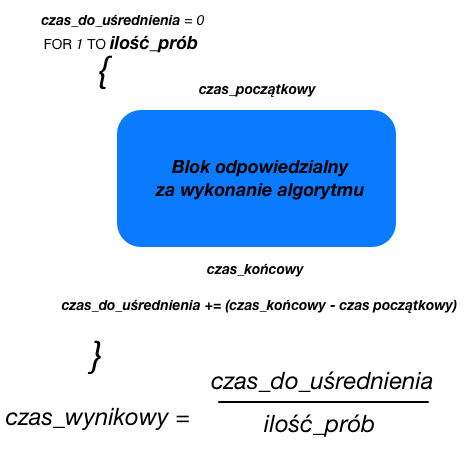
\includegraphics[width=0.5\textwidth]{tex/fig/time}
		\caption{Zarys pomiaru czasu podczas wykonywania algorytmu}
		\label{fig: time}
	\end{figure}

\end{enumerate}
Dokładna liczba iteracji zostanie dobrana metodą prób i błędów podczas wykonywania pomiarów.